\textbf{(CAP-COLUNI 2024 -- Q18)} No gráfico abaixo é apresentada, de modo aproximado, a evolução da área média das residências norte americanas durante o período de 1973 a 2003.

\begin{center}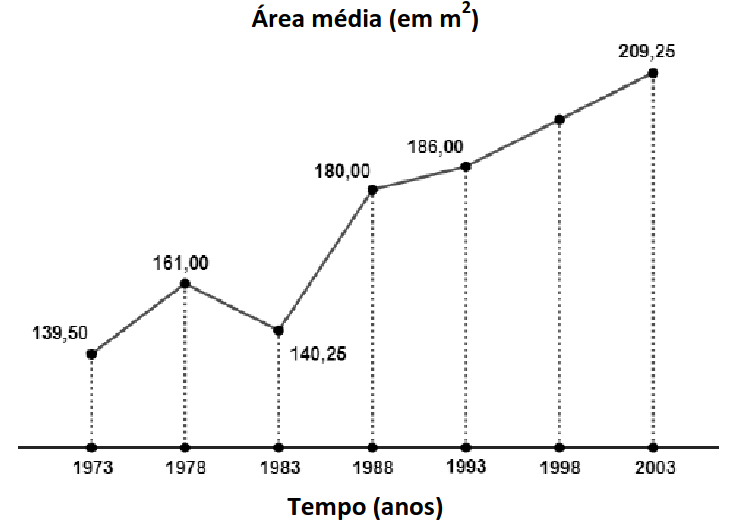
\includegraphics[width=0.58\linewidth]{static/simulados/coluni/latex-figs/2024-Q18.png}\end{center}

HOUSEL, Morgan. A psicologia financeira. 1. Ed. Rio de Janeiro. Harper Collins, 2021. p. 292.

Considere que no período entre os anos 1993 e 2003 o gráfico apresenta a mesma taxa de crescimento. Usando $\sqrt3\approx1{,}7$ e $\pi\approx3{,}1$, a área média aproximada de uma residência norte americana, no ano de 1998, está mais próxima da área de um:


\begin{enumerate}
	\item quadrado de lado medindo 16 m.
	\item triângulo equilátero de lado medindo 21 m.
	\item círculo de raio medindo 7 m.
	\item trapézio de bases medindo 10 m e 14 m, e altura medindo 12 m.
\end{enumerate}
